\section{Git strategy} \label{git_strategy}
	
\noindent \textbf{NOTE:} The first part of the actual Git history is not represented here accurately, as we were still refining our approach. This diagram showcases the idealized approach we have adopted and are using moving forward. It combines real elements from our Git history with some fictional commits and branches to illustrate key concepts concisely. Most merges are simplified into single arrows for clarity, and commit messages are omitted for brevity and focus.

\subsection{Tweaked Git Flow Strategy Overview}

``Tweaked Git Flow'' is a customized branching strategy designed to meet our team's specific project management needs. It integrates conventional commits and precise branch naming conventions to ensure clarity and traceability throughout the development and release lifecycle.

\subsection{Branch Types in Tweaked Git Flow}

\begin{enumerate}
	\item \textbf{Stable Branch (\texttt{stable})}
	\begin{itemize}
		\item \textbf{Purpose}: Represents the stable production-ready state of the codebase.
		\item \textbf{Workflow}:
		\begin{itemize}
			\item Reflects the latest stable release.
			\item Merges from \texttt{develop} for approved updates or critical fixes.
			\item Tags releases for deployment.
		\end{itemize}
	\end{itemize}
	
	\item \textbf{Hotfix Branches (\texttt{hotfix/})}
	\begin{itemize}
		\item \textbf{Purpose}: Fixes critical production issues.
		\item \textbf{Naming Convention}: \texttt{hotfix/103-login-api-bypass-fix}
		\item \textbf{Workflow}:
		\begin{itemize}
			\item Create from \texttt{stable}.
			\item Merge into \texttt{stable} and \texttt{develop} after validation.
		\end{itemize}
	\end{itemize}
	
	\item \textbf{Release Branches (\texttt{release/})}
	\begin{itemize}
		\item \textbf{Purpose}: Prepares for a new production release.
		\item \textbf{Naming Convention}: \texttt{release/1-D1}, \texttt{release/100-0.1.0}
		\item \textbf{Workflow}:
		\begin{itemize}
			\item Create from \texttt{develop}.
			\item Finalize the release (versioning, tagging).
			\item Merge into \texttt{stable} and \texttt{develop} after testing and validation.
		\end{itemize}
	\end{itemize}
	
	\item \textbf{Develop Branch (\texttt{develop})}
	\begin{itemize}
		\item \textbf{Purpose}: Integration branch for ongoing development.
		\item \textbf{Workflow}:
		\begin{itemize}
			\item Branch off from \texttt{main} (or \texttt{stable} for initial setup).
			\item Merges feature, bugfix, and documentation branches.
			\item Prepares releases (\texttt{release/} branches).
		\end{itemize}
	\end{itemize}
	
	\item \textbf{Documentation Branches (\texttt{docs/})}
	\begin{itemize}
		\item \textbf{Purpose}: Updates or enhances documentation and documents.
		\item \textbf{Naming Convention}: \texttt{docs/22-definition-of-tests}, \texttt{docs/23-git-strategy}
		\item \textbf{Workflow}:
		\begin{itemize}
			\item Create from \texttt{develop}.
			\item Merge into \texttt{develop} after updates.
		\end{itemize}
	\end{itemize}
	
	\item \textbf{Feature Branches (\texttt{feat/})}
	\begin{itemize}
		\item \textbf{Purpose}: Develops new features or significant changes.
		\item \textbf{Naming Convention}: \texttt{feat/101-login-api}
		\item \textbf{Workflow}:
		\begin{itemize}
			\item Create from \texttt{develop}.
			\item Merge into \texttt{develop} after completion.
		\end{itemize}
	\end{itemize}
\end{enumerate}

\subsection{Conventional Commits in Tweaked Git Flow}

Conventional commits provide a structured format for commit messages, facilitating clear communication and automated release notes generation. Each commit message follows the format \texttt{<type>: <description>}, where \texttt{<type>} indicates the nature of the change. Here are the commit types and their corresponding branch types in our ``Tweaked Git Flow'' strategy:

\begin{itemize}
	\item \textbf{hotfix}: Fixes critical production issues.
	\begin{itemize}
		\item Corresponding branch type: \texttt{hotfix/103-login-api-bypass-fix}
	\end{itemize}
	\item \textbf{release}: Prepares for a new production release.
	\begin{itemize}
		\item Corresponding branch types: \texttt{release/1-D1}, \texttt{release/100-0.1.0}
	\end{itemize}
	\item \textbf{docs}: Updates or enhances documentation.
	\begin{itemize}
		\item Corresponding branch types: \texttt{docs/22-definition-of-tests}, \texttt{docs/23-git-strategy}
	\end{itemize}
	\item \textbf{feat}: Used for new feature additions.
	\begin{itemize}
		\item Corresponding branch type: \texttt{feat/101-login-api}
	\end{itemize}
	\item \textbf{fix}: Addresses specific bugs.
	\begin{itemize}
		\item Corresponding branch type: \texttt{fix/102-wrong-email-type-in-login-api}
	\end{itemize}
\end{itemize}
	
\subsection{Tweaked Git Flow Strategy Overview}

\noindent \textbf{NOTE:} The first part of the actual Git history is not represented here accurately, as we were still refining our approach. This diagram showcases the idealized approach we have adopted and are using moving forward. It combines real elements from our Git history with some fictional commits and branches to illustrate key concepts concisely. Most merges are simplified into single arrows for clarity, and commit messages are omitted for brevity and focus.

\begin{figure}[h]
	\centering
	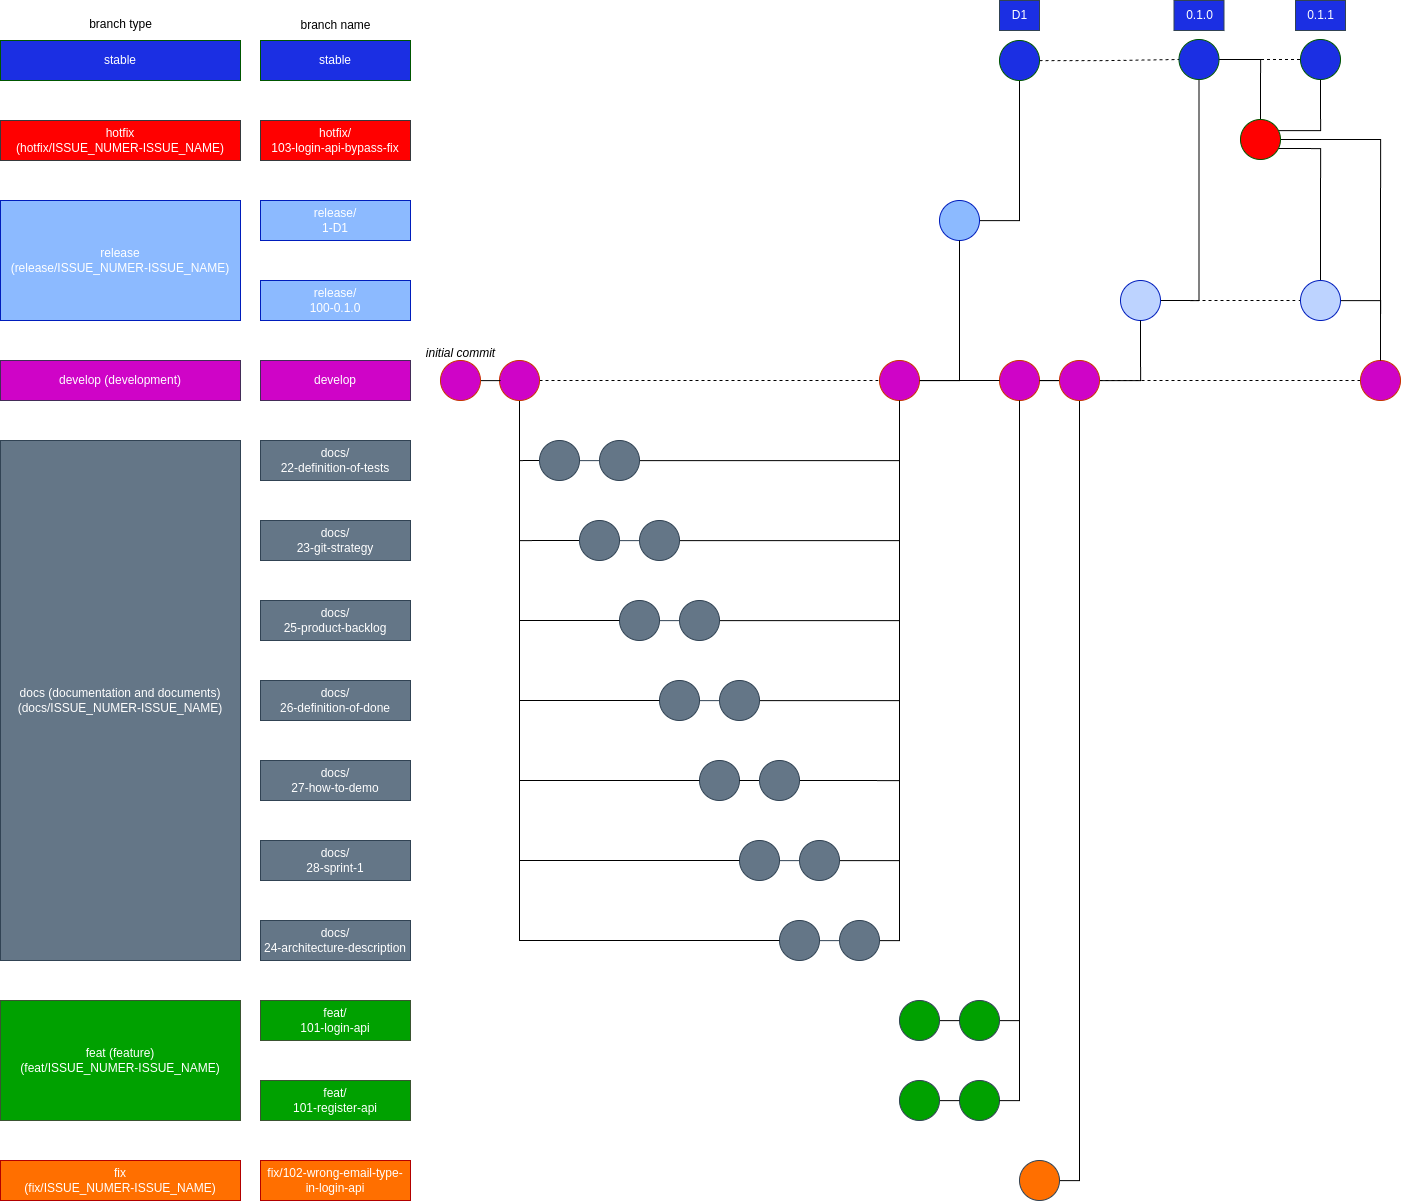
\includegraphics[width=0.9\textwidth]{images/git-strategy.png}
	\caption{Git strategy example graphic visualization}
\end{figure}

``Tweaked Git Flow'' is a customized branching strategy designed to meet our team's specific project management needs. It integrates conventional commits and precise branch naming conventions to ensure clarity and traceability throughout the development and release lifecycle.

\subsection{Branch Types in Tweaked Git Flow}

\begin{enumerate}
	\item \textbf{Stable Branch (\texttt{stable})}
	\begin{itemize}
		\item \textbf{Purpose}: Represents the stable production-ready state of the codebase.
		\item \textbf{Workflow}:
		\begin{itemize}
			\item Reflects the latest stable release.
			\item Merges from \texttt{develop} for approved updates or critical fixes.
			\item Tags releases for deployment.
		\end{itemize}
	\end{itemize}
	
	\item \textbf{Hotfix Branches (\texttt{hotfix/})}
	\begin{itemize}
		\item \textbf{Purpose}: Fixes critical production issues.
		\item \textbf{Naming Convention}: \texttt{hotfix/103-login-api-bypass-fix}
		\item \textbf{Workflow}:
		\begin{itemize}
			\item Create from \texttt{stable}.
			\item Merge into \texttt{stable} and \texttt{develop} after validation.
		\end{itemize}
	\end{itemize}
	
	\item \textbf{Release Branches (\texttt{release/})}
	\begin{itemize}
		\item \textbf{Purpose}: Prepares for a new production release.
		\item \textbf{Naming Convention}: \texttt{release/1-D1}, \texttt{release/100-0.1.0}
		\item \textbf{Workflow}:
		\begin{itemize}
			\item Create from \texttt{develop}.
			\item Finalize the release (versioning, tagging).
			\item Merge into \texttt{stable} and \texttt{develop} after testing and validation.
		\end{itemize}
	\end{itemize}
	
	\item \textbf{Develop Branch (\texttt{develop})}
	\begin{itemize}
		\item \textbf{Purpose}: Integration branch for ongoing development.
		\item \textbf{Workflow}:
		\begin{itemize}
			\item Branch off from \texttt{main} (or \texttt{stable} for initial setup).
			\item Merges feature, bugfix, and documentation branches.
			\item Prepares releases (\texttt{release/} branches).
		\end{itemize}
	\end{itemize}
	
	\item \textbf{Documentation Branches (\texttt{docs/})}
	\begin{itemize}
		\item \textbf{Purpose}: Updates or enhances documentation and documents.
		\item \textbf{Naming Convention}: \texttt{docs/22-definition-of-tests}, \texttt{docs/23-git-strategy}
		\item \textbf{Workflow}:
		\begin{itemize}
			\item Create from \texttt{develop}.
			\item Merge into \texttt{develop} after updates.
		\end{itemize}
	\end{itemize}
	
	\item \textbf{Feature Branches (\texttt{feat/})}
	\begin{itemize}
		\item \textbf{Purpose}: Develops new features or significant changes.
		\item \textbf{Naming Convention}: \texttt{feat/101-login-api}
		\item \textbf{Workflow}:
		\begin{itemize}
			\item Create from \texttt{develop}.
			\item Merge into \texttt{develop} after completion.
		\end{itemize}
	\end{itemize}
\end{enumerate}

\subsection{Conventional Commits in Tweaked Git Flow}

Conventional commits provide a structured format for commit messages, facilitating clear communication and automated release notes generation. Each commit message follows the format \texttt{<type>: <description>}, where \texttt{<type>} indicates the nature of the change. Here are the commit types and their corresponding branch types in our ``Tweaked Git Flow'' strategy:

\begin{itemize}
	\item \textbf{hotfix}: Fixes critical production issues.
	\begin{itemize}
		\item Corresponding branch type: \texttt{hotfix/103-login-api-bypass-fix}
	\end{itemize}
	\item \textbf{release}: Prepares for a new production release.
	\begin{itemize}
		\item Corresponding branch types: \texttt{release/1-D1}, \texttt{release/100-0.1.0}
	\end{itemize}
	\item \textbf{docs}: Updates or enhances documentation.
	\begin{itemize}
		\item Corresponding branch types: \texttt{docs/22-definition-of-tests}, \texttt{docs/23-git-strategy}
	\end{itemize}
	\item \textbf{feat}: Used for new feature additions.
	\begin{itemize}
		\item Corresponding branch type: \texttt{feat/101-login-api}
	\end{itemize}
	\item \textbf{fix}: Addresses specific bugs.
	\begin{itemize}
		\item Corresponding branch type: \texttt{fix/102-wrong-email-type-in-login-api}
	\end{itemize}
\end{itemize}
